\chapter{Literature Reviews}	
\label{chapter3}

%%% section 1
\section{Figure}

\paragraph{

The figure numbers shall represent the chapter numbers. For example, the first figure in \autoref{chapter3} shall be ``\autoref{chap3:fig:model}'', etc. the number and title of a figure (Figure caption) should be placed BELOW the figure. For the figure caption which contains only 1 line, it should align CENTER throughout the thesis. For the figure caption which contains more than 1 line, it should align left throughout the thesis. The figure format should be pdf, png, jpg or \lstinline[language=C]!\chemfig! as \autoref{chap3:fig:mychemfig}


}

%%%%%%%%%%%%%%%%%%%%%%%%% FIGURE BEGIN %%%%%%%%%%%%%%%%%%%%%%%%% 
\begin{figure}[ht]
\centering
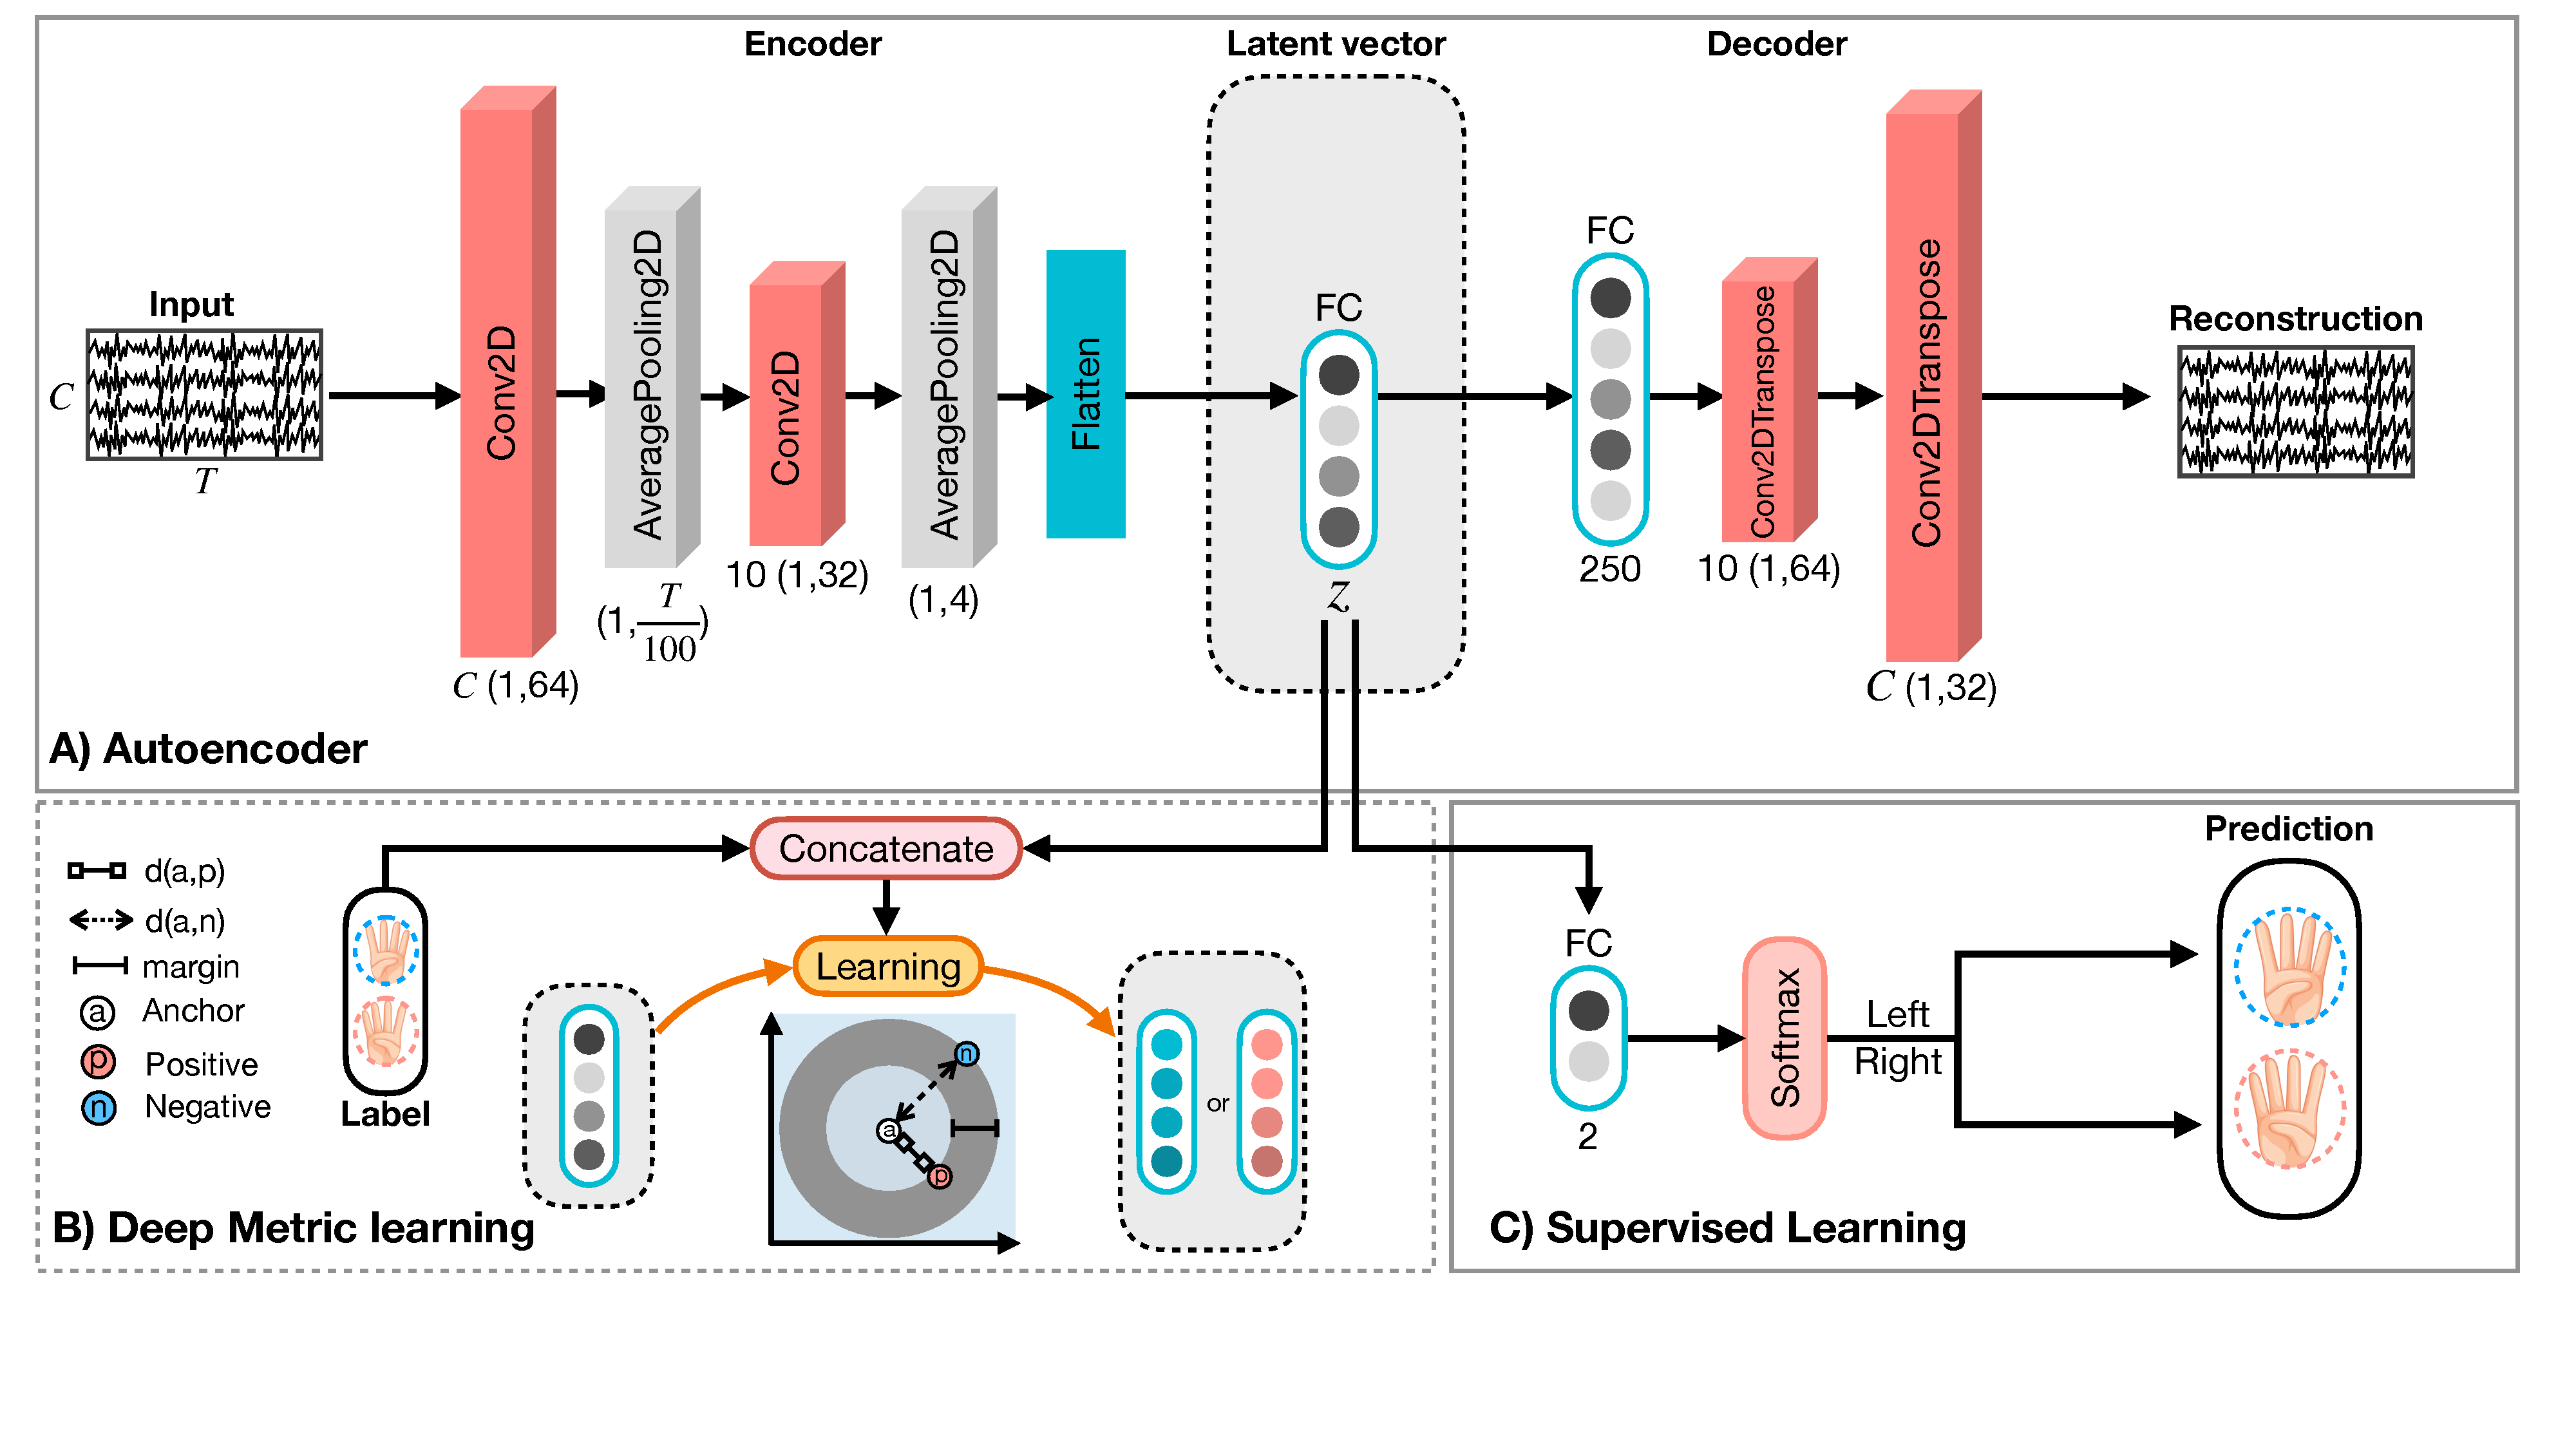
\includegraphics[width=1\columnwidth]{figures/ch3/model.pdf}
\longcaption[long caption: The MIN2Net model architecture.]{\lipsum[1]}
\label{chap3:fig:model}
\end{figure}
%%%%%%%%%%%%%%%%%%%%%%%%% FIGURE END %%%%%%%%%%%%%%%%%%%%%%%%% 


%%%%%%%%%%%%%%%%%%%%%%%%% FIGURE BEGIN %%%%%%%%%%%%%%%%%%%%%%%%% 
\begin{figure}[ht]
    \centering
    % From the documentation
    % https://ctan.mirror.garr.it/mirrors/ctan/macros/generic/chemfig/chemfig-en.pdf
    \chemnameinit{\chemfig{R-C(-[:-30]OH)=[:30]O}}
    \schemestart
    \chemname{\chemfig{R’OH}}{Alcohol}
    \+
    \chemname{\chemfig{R-C(-[:-30]OH)=[:30]O}}{Carboxylic acid}
    \arrow(.mid east--.mid west)
    \chemname{\chemfig{R-C(-[:-30]OR’)=[:30]O}}{Ester}
    \+
    \chemname{\chemfig{H_2O}}{Water}
    \schemestop
    \chemnameinit{}
    \caption{The caption on this figure, the second and other lines need to be aligned with the first letter of the first line.}
    \label{chap3:fig:mychemfig}
\end{figure}

%%%%%%%%%%%%%%%%%%%%%%%%% FIGURE END %%%%%%%%%%%%%%%%%%%%%%%%% 


\section{Morbi dolor nulla, malesuada eu}

\paragraph{
\lipsum[1] % just dummy text
}
